

\begin{wrapfigure}{l}{0.2\textwidth}
\centerline{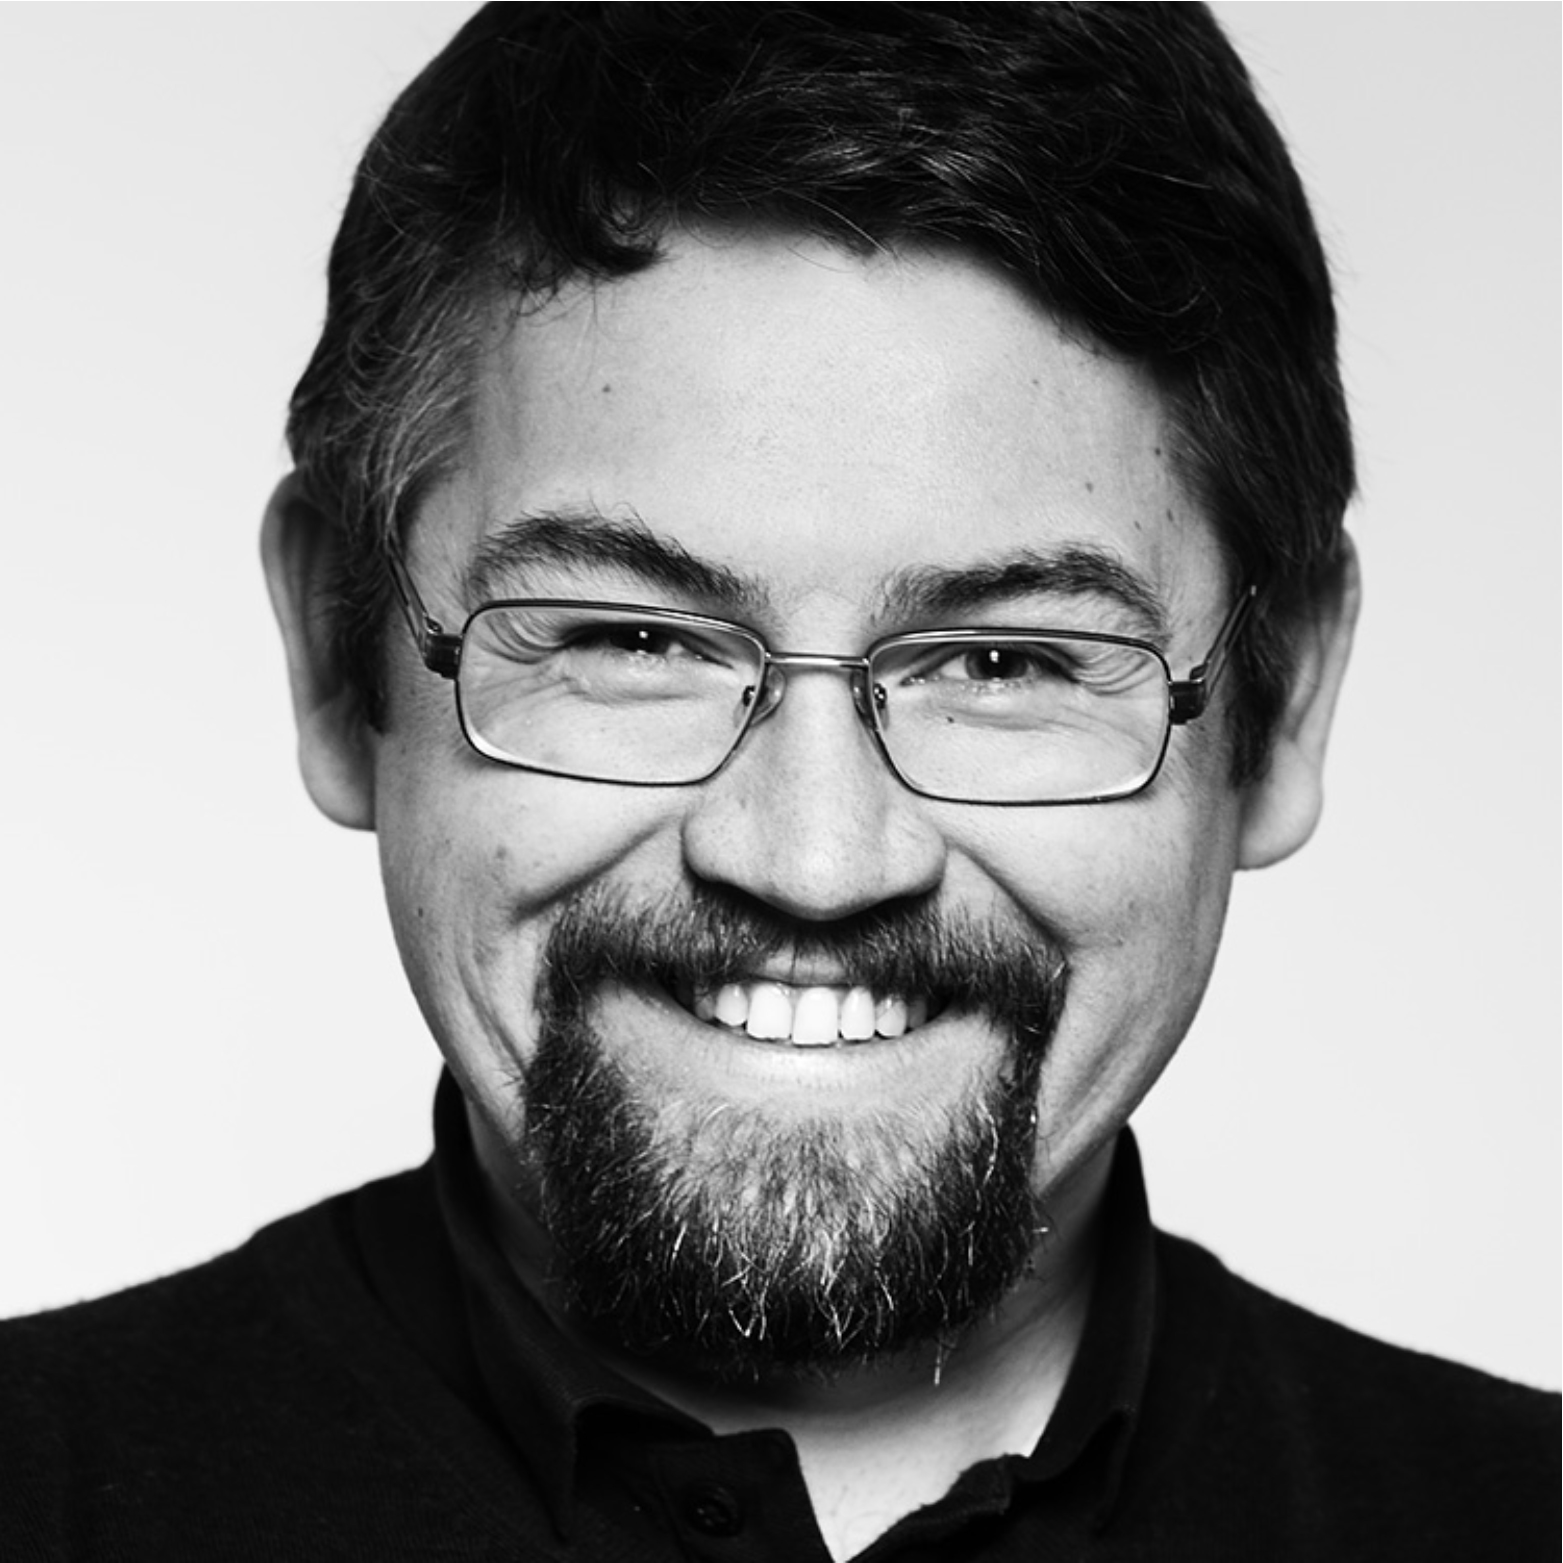
\includegraphics[width=30mm]{wulff} }
\end{wrapfigure}

 \textbf{Carsten Wulff}
received the M.Sc. and Ph.D. degrees in
electrical engineering from the Department of Electronics and Telecommunication, Norwegian University of Science and Technology (NTNU),
in 2002 and 2008, respectively.
During his Ph.D. work at NTNU, he worked on open-loop sigma-delta
modulators and analog-to-digital converters in nanoscale CMOS
technologies. In 2006-2007, he was a Visiting Researcher with the
Department of Electrical and Computer Engineering, University of
Toronto, Toronto, ON, Canada. He is currently the Group Manager for the
Wireless Group at Nordic Semiconductor ASA, Trondheim, Norway and a
Post Doctoral fellow at NTNU. His
present research interests includes analog and mixed-signal CMOS
design, design of high-efficiency analog-to-digital converters and
low-power wireless transceivers. He is the developer of Custom IC
Compiler, a general purpose integrated circuit compiler.
